\documentclass{llncs}
\usepackage{amssymb}
\usepackage{graphicx}
\usepackage[ruled,linesnumbered,boxed]{algorithm2e}
\usepackage{graphicx}
\usepackage{amsmath}
%\usepackage{mathtools}
%\usepackage{color}
\usepackage{tabularx}
\usepackage[colorlinks, linkcolor=blue, anchorcolor=blue, citecolor=green]{hyperref}
%\usepackage{booktabs}
\usepackage[table]{xcolor}
%\uespackage{colortbl}
\usepackage[tight,footnotesize]{subfigure}
\usepackage{booktabs}
\usepackage{fancyhdr}
\usepackage{lastpage}
\usepackage{layout}
\usepackage{here}
%\usepackage{ctex}

%\footskip = 10pt
\pagestyle{fancy}
\chead{Group Project}
\lhead{CS214-Algorithm@SJTU}
\rhead{Instructor: Xiaofeng Gao, Lei Wang}
\rfoot{}
\cfoot{Page \thepage \ of \pageref{LastPage}}
\addtolength{\headheight}{0.5\baselineskip}
\addtolength{\headwidth}{0\marginparsep}
\addtolength{\headwidth}{0\marginparwidth}



\title{Scheduling Jobs across Geo-Distributed Data Centers}
\subtitle{Project for Algorithm and Complexity \vspace{-3mm}}

\author{Jiaqi Pan (519030910243, 2123371072@qq.com), \\Ran Gao (519030910223, gaoran2993@sjtu.edu.cn), \\Beichen Yu (519030910245, polarisybc@sjtu.edu.cn)}
\institute{Shanghai Jiao Tong University, Shanghai, China}

\begin{document}
\bibliographystyle{splncs}

%\linespread{0.85}

%==============================================================================
\maketitle
\begin{abstract}\vspace{-5mm}
    In this paper, we propose an algorithm based on \textbf{0-1 integer linear programming (ILP)} to solve the problem of scheduling Jobs across geo-distributed data centers. ~\\

    First of all, we formalized the problem to a minimize problem. In particular, to achieve the \textbf{max-min fairness}, we strengthen it to minimize a sequence in lexicographic order.~\\
    
    Second, we proved the \textbf{NP-completeness} of the problem. We convert this scheduling problem for multiple times, and finally we prove that it can reduce from 3-SAT problem.~\\
    
    After that, we try to find an algorithm to solve the problem. We first proposed a feasible algorithm with the idea of greedy, and analyze whether it is optimal. Then we established a model based on integer linear programming through analysis, propose an algorithm to find the optimal scheduling plan, and further expand the algorithm on this basis to solve the max-min fairness.~\\
    
    At last, in order to solve the problem of interdependence between tasks, we use \textbf{DAG schedule} to eliminate dependencies,and determined the specific process to solve the problem.    ~\\

\textbf{Keywords:} max-min fairness, NP-completeness, ILP, DAG schedule.
\end{abstract}

\section{Background}

In multiple data centers around the world, it is increasingly common to generate and process large amounts of data distributed geographically. Data analysis tasks are usually carried out in successive calculation stages, and each stage is composed of multiple parallel calculation tasks. To start a new calculation phase, the intermediate data of the previous phase needs to be extracted, which may start multiple network streams.

When the input data is located in multiple data centers, a simple method is to collect all the data to be processed locally in a single data center. Naturally, transferring large amounts of data across data centers can be slow and inefficient because of the limited bandwidth on the network links between data centers. Existing research shows that if the tasks in the analysis job can be distributed in various data centers and closer to the data to be processed, better performance can be achieved. In this case, it is very important to design the best task allocation strategy to allocate tasks to the data center, because different strategies will lead to different flow patterns between data centers and ultimately lead to different job completion times. However, when designing the optimal task allocation strategy, one cannot only consider a single data analysis job. The problem of distributing tasks belonging to multiple jobs across data centers still exists. Due to the limited amount of resources in each data center, multiple jobs would have competed with each other for resources. Therefore, it is very important to maintain fairness when assigning such a shared resource pool. If the tasks of one job are assigned without considering other jobs, this cannot be achieved.

The design goal of this article is to calculate the best way to distribute tasks belonging to multiple jobs to geographically distributed data centers, so that all jobs can achieve the possible completion time without affecting the performance of other jobs. Best performance. For each job, different task assignments will result in different sizes of streams, flowing through different links, resulting in different job completion times. In addition, these jobs will definitely share and compete for the same computing resource pool among these data centers. In order for these tasks to achieve the best performance, we need to consider how to arrange their tasks together rather than independently. This means that we need to achieve Max-Min fairness between jobs in the shared data center. More specifically, we want to minimize the job completion time of all concurrent jobs while maintaining Max-Min fairness. 

\section{Nomenclature}
In this paper we use the nomenclature in Table \ref{tab:Nomen} to descibe our model. Other symbols that are used only once will be described later.

\begin{table}[H]
    \centering
    \caption{Nomenclature}
    \label{tab:Nomen}
    \begin{tabular}{c|p{14cm}}
\toprule
    	Symbol & Definition\\
\midrule
	$K$ & The job set\\
	$D$ & The data center set\\
	$T_k$ & The sub tasks set of job $ k $\\
	$a_d$ & The number of available computing slots in data center $ d $\\
	$t_k$ & The total time that job $ k $ spends\\
	$b_{ij}$ & The bandwidth between data center $ i $ and data center $ j $\\
	$S_{k,i}$ & The data center set of the data source for the $ i $-th sub-task of job $ k $\\
	$d_{k,i,s}$ & The amount of data needed for the $ i $-th sub-task of job $ k $ to get from data center $ s $\\
	$\tau$ & The time sequence of the total time for all jobs in descending order\\
	$c_{k,i,j}$ & The transmission time for $ tsk_{i} \in T_k $ of job $ k $ assigned on the data center $ j $\\
	$e_{k,i,j}$ & The execution time for $ tsk_{i} \in T_k $ of job $ k $ assigned on the data center $ j $\\
	$x_{k,i,j}$ & The binary variable of whether $ tsk_{i} \in T_k $ of job $ k $ is assigned on the data center $ j $\\
	$f(k,i,j)$ & Equal to $ x_{k,i,j}(c_{k,i,j} + e_{k,i,j}) $\\
	
\bottomrule   \end{tabular}
\end{table}

\section{Formalization of the Problem}

\subsection{Multi-job Scheduling Problem}

\begin{itemize}
    \item In the problem, we have a series of jobs $ K = \{1, 2, \cdots, k_n\} $ waiting for completion. 
    
    \item The source of the data for these jobs is not centrally managed, but is distributed in many different data centers $ D = \{1, 2, \cdots, d_n\} $. 
    
    \item For each job $ k \in K $, there are a set of sub tasks $ T_k = \{tsk_1, tsk_2, \cdots, tsk_{k_n}\} $. We need to pay attention that these tasks are not necessarily parallel. There will be dependencies on data sources between different tasks.  
    
    \item The tasks must be executed on the computing slots in the data center. The number of available computing slots in each data center is limited. We use $ a_d $ to denote the number of available computing slots in data center $ d $. 
    \item For each job, we denote $ t_k $ as the total time job $ k $ spends. The total time here includes the sum of transmission time and execution time. Only when all the sub-tasks of job $ k $ are completed, the timing is completed.
    \item During data transmission, it issues involving transmission bandwidth. We use $ b_{ij} $ to represent the bandwidth between data center $ i $ and data center $ j $. We need to pay attention that $ b_{ij} $ is not necessarily equal to $ b_{ji} $, because the bandwidth in both directions is not necessarily the same.
    \item During data transmission, another key point is data. For the $ i $-th sub-task of job $ k $, the data center set of the data source it needs is represented by $ S_{k,i} $. And for each $ s \in S_{k,i} $, the amount of data is denoted as $ d_{k,i,s} $.
\end{itemize}

Our purpose is very clear. We need to find a scheduling solution to minimize $ \mathop{max}\limits_{k \in K} \{ t_k \} $. 

\subsection{Max-Min Fairness in this Problem}

This question puts an additional request on us: we want the resource to be allocated fairly. In other words, we need to satisfy the max-min fairness of scheduling.

For each job $ k $ in $ K $, we have a total time $ t_k $. Sort these times from longest to shortest, and we get a time sequence:
 $$ \tau = <t^{\prime}_1,t^{\prime}_2, \cdots, t^{\prime}_{kn}> , t^{\prime}_1 \geqslant t^{\prime}_2 \geqslant \cdots \geqslant t^{\prime}_{k_n}$$.

We use the lexicographic order of this time series to characterize the max-min fairness. Assume $ \tau $ and $ \tau^{\prime} $ are two time sequence of different scheduling plans. If $ \tau \leqslant_{lex} \tau^{\prime} $, we can conclude that the former scheduling plan is fairer than the latter. 

In order to achieve the max-min fairness, we need find the minimal time sequence in lexicographic order. In other word, we need to:

$$ \min\limits_{lex}  \tau = <t^{\prime}_1,t^{\prime}_2, \cdots, t^{\prime}_{kn}> , t^{\prime}_1 \geqslant t^{\prime}_2 \geqslant \cdots \geqslant t^{\prime}_{k_n} $$.

\section{NP-Completeness of the Problem}

This problem is NP-complete.\\
\indent\setlength{\parindent}{2em} Based on the abstract and description, the project has strong comprehensiveness, covering a series of concepts. We can consider this problem as a integration of several individual sub-problems. And actually quite a few of them are NP-complete.\\
\indent\setlength{\parindent}{2em}On one hand, there are precedence constraints between tasks, with multiple stages. We use a directed acyclic graph (DAG) to show intuitively, where the nodes denote the tasks and edges denote the constraints. And in fact, scheduling jobs with multiprocessors in DAG with the objective of minimizing the job completion time is NP-complete\cite{ref_article2}.\\
\indent\setlength{\parindent}{2em}Below we prove it’s NP-complete.\\
\indent\setlength{\parindent}{2em}Let set $S$ denote the collection of all sub-tasks, which follow the constraints in DAG. That’s to say, if there is a directed edge from task $A$ to task $B$, then task $B$ must commence before the finish time of task $A$. And then, we can define a partial relation in $S$:\\
\indent\setlength{\parindent}{2em}If the execution of task $B$ is constrained by task $A$, then we have $A\prec B$.\\
\indent\setlength{\parindent}{2em}Now we can express the task scheduling problem algebraically, without the use of DAG:\\
\indent\setlength{\parindent}{2em}\textbf{\textit{Problem 1:[General scheduling problem]}}Given a set of $n$ tasks $S$, a partial relation $\prec$ on $S$, a weighting function $W$ on $S$ where $W(A)$ denotes the total time of task $A$, the number of processors $k$ and a time limit $T$, does there exist a total function $f$ from $S$ to $\{0, 1, ..., T-1\}$ where $f(A)$ denotes the start time of the task $A$, such that:\\
\indent\setlength{\parindent}{2em}(i). if $A\prec B$, then $f(A)+W(A)\leqslant f(B)$,\\
\indent\setlength{\parindent}{2em}(ii). for each $A$ in $S$, $f(A)+W(A)\leqslant T$,\\
\indent\setlength{\parindent}{2em}(iii). for each time point $t$, $0\leqslant t\leqslant T-1$, there are at most $k$ values of task $A$ for which $f(A)\leqslant t< f(A)+W(A)$.\\ 
\indent\setlength{\parindent}{2em}The problem is a decision problem, and if we change it to the form of a search problem for minimum completion time $T$, it becomes our project. And the general scheduling problem is proved to be NP-complete.\\
\indent\setlength{\parindent}{2em}Here we give a special situation of the problem, where for any task $A$ in $S$, $W(A)=1$. We call it
\textbf{\textit{Problem 2:[Single execution time scheduling]}}. Obviously, if it’s NP-complete, then the general problem is NP-complete, too. As for the single execution scheduling, we introduce a slightly more complex new problem based on it:\\
\indent\setlength{\parindent}{2em}\textbf{\textit{Problem 3:[Single execution time scheduling with variable number of processors]}}Given a set $S$ of $n$ tasks, a partial relation $\prec$ on $S$, a time limit $T$, and a sequence of integers $c_0,c_1,\cdots,c_{T-1}$, where $\sum\limits_{i=0}^{T-1}c_i=n$, does there exist a total function $f$ from $S$ to $\{0, 1, ..., T-1\}$ such that:\\
\indent\setlength{\parindent}{2em}(i). $f^{-1}(i)$ has exactly $c_i$ members,\\
\indent\setlength{\parindent}{2em}(ii). if $A\prec B$, then $f(A)<f(B)$.\\
\indent\setlength{\parindent}{2em}Now we prove that $\textit{Problem 3}\leq _p\textit{Problem 2}$.\\
\indent\setlength{\parindent}{2em}\textbf{\textit{Proof: }} Given a instance of \textit{Problem 3}, we introduce new tasks $I_{i,j}$, where $0\leqslant i<T$ and $0\leqslant j\leqslant n-c_i$. Let the old tasks be related by $\prec$ as before and let $I_{i,j}\prec I_{i+1,k}$ for $0\leqslant i<T-1$, arbitrary $j$ and $k$. Then we just provide $n+1$ processors, and we get a instance of \textit{Problem 2}, because for any $0\leqslant i<T$, and the $i-th$ time unit, we add exactly $n+1-c_i$ new tasks, and in total there are exactly $n+1$ tasks. So now the instance of \textit{Problem 2} has a solution if and only if the original instance of \textit{Problem 3} does. The construction from \textit{Problem 3} to \textit{Problem 2} needs at most $O(n^2)$ time, which means \textit{Problem 3} polynomial reduced to \textit{Problem 2}.\\
\indent\setlength{\parindent}{2em}As for \textit{Problem 3}, we can also prove that $\textit{3-SAT}\leq_p\textit{Problem 3}$.\\
\indent\setlength{\parindent}{2em}The proof is so long that we leave out the proof. Detailed proof can be found in related literature\cite{ref_article3}. \\
\indent\setlength{\parindent}{2em}Now we have $\textit{3-SAT}\leq_p\textit{Problem 3}\leq_p\textit{Problem 2}$. As we all know, \textit{3-SAT} is NP-complete, which indicates that \textit{Problem 2} is NP-complete. As \textit{Problem 2} is the sub-problem of \textit{Problem 1}, we can conclude that \textit{Problem 1} is also NP-complete. Equivalently, scheduling jobs with multiprocessors in DAG with the objective of minimizing the job completion time is NP-complete.\\
\indent\setlength{\parindent}{2em}On the other hand, to solve the problem, we introduce the binary variables to indicate the allocation of the tasks, transforming the problem to a 0-1 integer linear programming problem, which is also NP-complete (we can prove that \textit{3-SAT} Problem polynomial reduces to this problem).\\
\indent\setlength{\parindent}{2em}In addition, for such a scenario of multi-data-center parallel task execution, even single-server-single-queue versions of this scheduling problem have been shown to be strongly NP-hard\cite{ref_article4}. \\
\indent\setlength{\parindent}{2em}Above all, we come to the conclusion that this problem is NP-complete.\\
\\

\section{A Simple Greedy Algorithm}


To solve that problem, we first want to put forward a naive algorithm: a simple greedy algorithm to give a scheduling plan. 

Our idea is really simple. To ensure that the completion time of all tasks is minimized, we should guarantee that all the available slots in every data center remain busy. So for each slot, we set its two states: busy state and idle state. When a slot is in the idle state, we let it recursively find tasks that can be performed. 

This involves a scheduling problem. When a slot has multiple optional tasks to choose from, and when multiple slots select the same task at the same time, we should determine the order of scheduling in some way. We greedily use the SJF(Short Job First) algorithm for scheduling. When an idle slot has multiple tasks to choose from, it should calculate the sum of the transmission time and execution time of all these tasks to be selected, and choose the task with the shortest total time. In addition, if there are multiple slots competing for the same task at the same time, the task will be assigned to the slot with the shortest transmission time.

Here we can use multithreading to implement this algorithm to improve efficiency. Specifically, we need to assign a thread to each available slot to execute the above algorithm. Whenever a task is executed, the thread selects the thread with the shortest time from the current ready queue to execute next. This involves synchronization between threads, and mutual exclusion needs to be achieved by adding locks.

Although the greedy algorithm can indeed give us a solution, does this solution give the optimal solution? The answer is negative. Such an algorithm only pays attention to the operation of each slot, and does not perform scheduling from an overall perspective. It is easy for us to think of the following situation: A certain task is suitable for execution in a certain slot, but this task is still running at some time. But at this time, this slot can find a troublesome other task. 
At the same time, the requirement of Max-Min Fairness cannot be met when using this algorithm.

\section{Integer Linear Programming Algorithm}

\subsection{ILP Model Construction}
In order to minimize the scheduling time, we can use a 0-1 integer programming model\cite{ref_article1} to solve the problem. 

We need to maintain the status of the time spent by each task on different slots in order to filter from it. Denote $ c_{k,i,j} $ as the transmission time for $ tsk_{i} \in T_k $ of job $ k $ assigned on the data center $ j $. Then, we need to calculate the value of $ c_{k,i,j} $ for each $ i, j $ and $ k $. 

If the source data center happens to be the assigned data center, the transmission time can be omitted. Otherwise, the transmission time should be the quotient of the data amount and the bandwidth. We need to pay attention that if there are a series of data to transport from different data centers, the final transmission time should be the maximal one.  

$$ c_{k,i,j}=\left\{
\begin{aligned}
&0, &S_{k,i} = \{j\}. \\
&\max\limits_{s \in S_{k,i}} \frac{d_{k,i,s}}{b_{s,j}}, &\textrm{otherwise}.\\
\end{aligned}
\right.
$$

After that, if we use $ e_{k,i,j} $ to denote the execution time for $ tsk_{i} \in T_k $ of job $ k $ assigned on the data center $ j $, the total time of an assigned task is the sum of $ c_{k,i,j} $ and $ e_{k,i,j} $. 

Now we use a binary variable $ x_{k,i,j} $ to denote the assignment of tasks. If we assign $ tsk_{i} \in T_k $ of job $ k $ on data center $ j $, $ x_{k,i,j} = 1 $; otherwise  $ x_{k,i,j} = 0 $. 

For a job $ k $, its completion time is determined by the slowest task. So we have:

$$ t_k = \max\limits_{tsk_i \in T_k, j \in D} \{ x_{k,i,j}( c_{k,i,j}+e_{k,i,j}) \}$$

Then the final goal is connected with the binary assignment matrix $\mathbf{x}$. All we need to do is to modify this matrix to minimize time sequence $ \tau $ in lexicographic order. But there are some constraints. 

First, for each task, it can only be assign on an unique data center. That means for any $ k\in K $ and $ tsk_i \in T_k $, we have $ \sum\limits_{j \in D} x_{k,i,j} = 1$.

Second, we should never forget that the slots of data center are not infinite. So the number of tasks assigned to a data center should not larger than the number of its slots. That means that for any $ j \in D $, we have $  \sum\limits_{ k\in K } \sum\limits_{tsk_i \in T_k } x_{k,i,j} \leqslant a_j $.

Third, because $ x_{k,i,j} $ is a binary variable, so we have $ x_{k,i,j} \in \{0,1 \} $.

After clarifying the goals and constraints, we can write down our linear programming problem:

$$ \min\limits_{lex}  \tau = <t^{\prime}_1,t^{\prime}_2, \cdots, t^{\prime}_{kn}> , t^{\prime}_1 \geqslant t^{\prime}_2 \geqslant \cdots \geqslant t^{\prime}_{k_n} $$

s.t.
$$\left\{
\begin{aligned}  
    &t_k = \max\limits_{tsk_i \in T_k, j \in D} \{ x_{k,i,j}( c_{k,i,j}+e_{k,i,j}) \}, \forall k \in K\\
    &\sum\limits_{j \in D} x_{k,i,j} = 1, \forall k\in K ,\forall tsk_i \in T_k \\
    &\sum\limits_{ k\in K } \sum\limits_{tsk_i \in T_k } x_{k,i,j} \leqslant a_j, \forall j \in D  \\
    &x_{k,i,j} \in \{0,1 \},\forall k\in K ,\forall tsk_i \in T_k ,\forall j \in D  \\
\end{aligned}
\right.
$$

\subsection{ILP Model Based Solution}

First, we try to solve the problem not considering the max-min fairness. That means we need to solve that problem:

$$min \quad \mathop{max}\limits_{k \in K} \{ t_k \} $$ 

with the same constraints.

Generally speaking, the ILP problem is proved to be a NP-complete problem. But we can try to use a Monte Carlo method to solve the ILP problem.

According to the constraint  $\sum\limits_{j \in D} x_{k,i,j} = 1, \forall k\in K ,\forall tsk_i \in T_k $, for this three-dimensional matrix $\mathbf{x}$, there is only one element can equal one if $ i $ and $ k $ are fixed. According to this feature, we establish a two-layer loop for $i$ and $k$, and choose a data center $ j $ completely randomly. We set $ x_{k,i,j} = 1 $, and $\forall j^* \in D, j^* \neq j, x_{i,j^*,k} = 0 $. In this way, we have generated the distribution matrix $ \mathbf{x} $ through the Monte Carlo method.

The next thing we need to do is only two steps. First, we need to examine that whether the another constraint $ \sum\limits_{ k\in K } \sum\limits_{tsk_i \in T_k } x_{k,i,j} \leqslant a_j, \forall j \in D  $ is satisfied. If it is surely satisfied, the matrix $\mathbf{x}$ is valid. Then we can calculate the $ \mathop{max}\limits_{k \in K} \{ t_k \}  $. We need to repeat the above method many times, record the result corresponding to the matrix obtained by each Monte Carlo method and find the one with the smallest result. The corresponding matrix $ \mathbf{x} $ is the corresponding scheduling plan we want.

After this ILP problem is solved, we further consider the max-min fairness. Our idea is that, every time after solving the sub-problem with the longest time, we fix it, and repeat the algorithm to solve the sub-problem with the second longest time.

Specifically, first we should find the task which is the slowest, because this task determines the completion time of the entire project. That means we need to find the $  x_{k^*,i^*,j^*} $ that the completion time $ f(k^*,i^*,j^*) =  x_{k^*,i^*,j^*}(c_{k^*,i^*,j^*}+e_{k^*,i^*,j^*}) $ is the maximal. 

The adjustment work is divided into the following steps: first, we need to fix $  x_{k^*,i^*,j^*} = 1 $. Second, as $ tsk_{i^*} $ is be assigned to $ j^* $, we have $  x_{k^*,i^*,j} = 0, j \in D, j \neq j^* $. Third, the task is assigned means that one slot of data center $ j $ is occupied. We should rewrite the constraint into $ \sum\limits_{ k\in K } \sum\limits_{tsk_i \in T_k (k,i) \neq (k^*,i^*) } x_{k,i,j^*} \leqslant a_j^*  - 1$. Finally, we need to modify the completion time of other tasks of the job $ f(k^*,i,j) $ to $  x_{k^*,i^*,j^*}(c_{k^*,i^*,j^*}+e_{k^*,i^*,j^*}) $. Then we can assure that job $ k $ is modified. We then repeat the ILP problem until all jobs are modified. In this way, the max-min fairness is satisfied.

The pseudo code of the overall algorithm is as follows:

\begin{minipage}[t]{0.8\textwidth}
    \begin{algorithm}[H]
        \BlankLine
        \caption{ILP Model Based Algorithm}
        Initialize a job set $ K^{\prime} = K $;

        \While{$K^{\prime} \neq \varnothing$}
        {
            Using Monte Carlo method to solve the sub-problem;\\
            Find $x_{k^*,i^*,j^*}$ that maximize $ f(k^*,i^*,j^*) $;\\
            Fix $x_{k^*,i^*,j^*} = 1$ and  $x_{k^*,i^*,j} = 0, j \neq j^*$;\\
            Rewrite the slots constraint into $ \sum\limits_{ k\in K } \sum\limits_{tsk_i \in T_k (k,i) \neq (k^*,i^*) } x_{k,i,j^*} \leqslant a_j^*  - 1$;\\
            Modify $ f(k^*,i,j) =  x_{k^*,i^*,j^*}(c_{k^*,i^*,j^*}+e_{k^*,i^*,j^*}) $;\\
            Remove $ k^* $ from $ K^{\prime} $;
        }
        
    \end{algorithm}
    \end{minipage}

\subsection{Complexity Analysis}

Let's perform complexity analysis below.

First analyze the space complexity, which is relatively simple. $  x_{k,i,j} $, $ c_{k,i,j} $ and $ e_{k,i,j} $ are the arrays we created. So the space complexity is $ O(|K||T_k|_{max}|D|) $.

Then we analyze the time complexity. Obviously the time complexity of this problem cannot be polynomial, and it is also more complicated to analyze. Since we are using Monte Carlo method, suppose the number of times to obtain a matrix $ \mathbf{x} $ that satisfies all constraints is $ X $, then the time complexity of each process of finding the minimum $  \mathop{max}\limits_{k \in K} \{ t_k \} $ is $ O(X|K||T_k|_{max}|D|) $. In order to achieve the max-min fairness, we use the  Monte Carlo method for $ |K| $ times, so we can make sure that the time complexity is $ O(X|K|^2|T_k|_{max}|D|) $.

\section{Precedence Constraint Relief: DAG schedule}

Although we have already come up with an algorithm to solve this problem, we cannot directly use it to solve our problems. That is because there are precedence constraints between tasks of a job. If a task requires data from other tasks, it must wait until the task it depends on is finally completed.

Now we try to eliminate this dependency in order to use our algorithm normally.

We can use a directed acyclic graph (DAG) to represent a job. Each node in the DAG represents a task, and each directed edge represents a precedence constraint. For example, the DAG of the toy data is shown below.

\begin{figure}[H]
    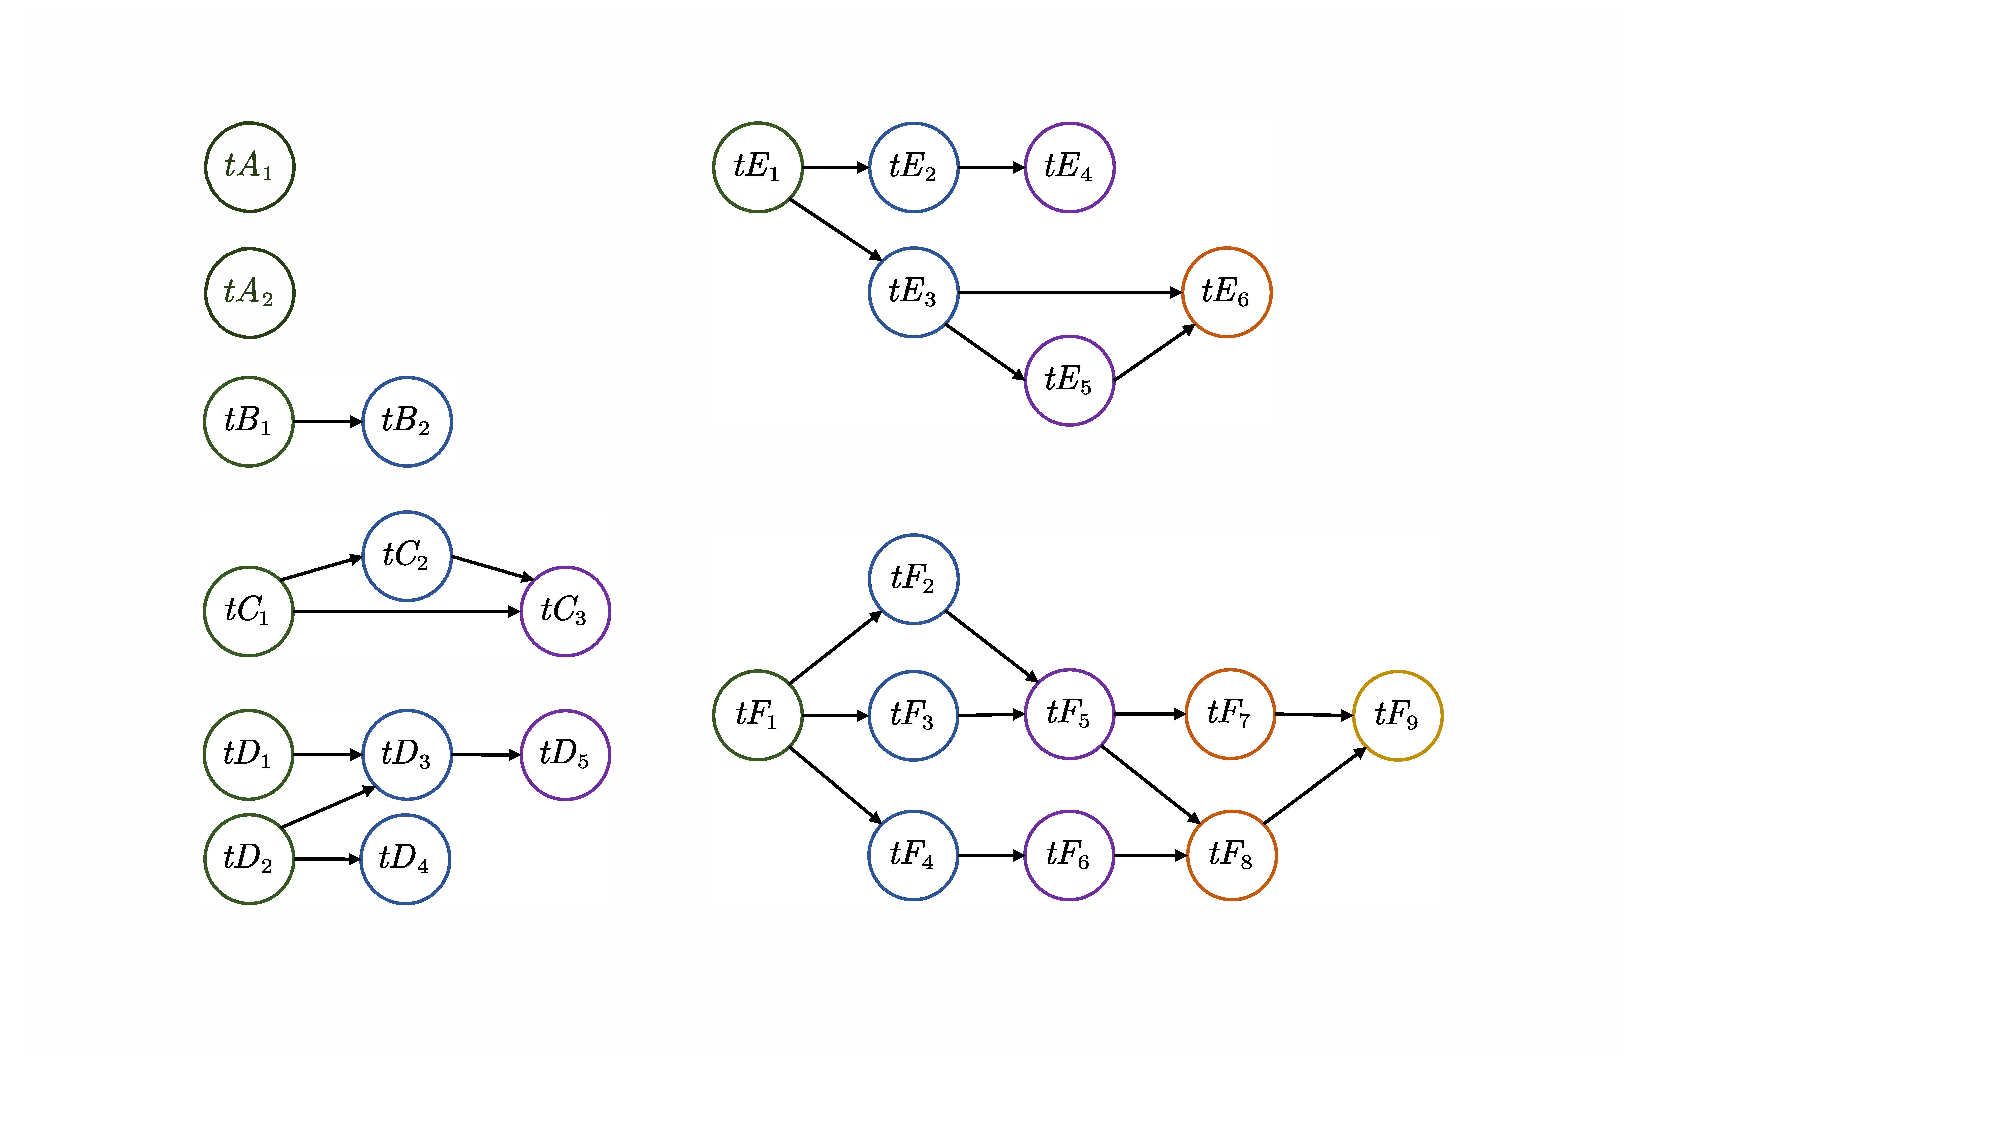
\includegraphics[width=0.8\textwidth]{DAG.pdf}
    \centering
    \caption{the DAG of the Toy Data} 
    \end{figure}

Our idea is to set up a task pool. All tasks in the task pool are parallel and there are no dependencies between each other. And our algorithm is responsible for scheduling these parallel tasks in the process pool. At the same time, we need to implement a DAG scheduler, which is used to submit all the tasks that not dependent on each other.

\begin{figure}[H]
    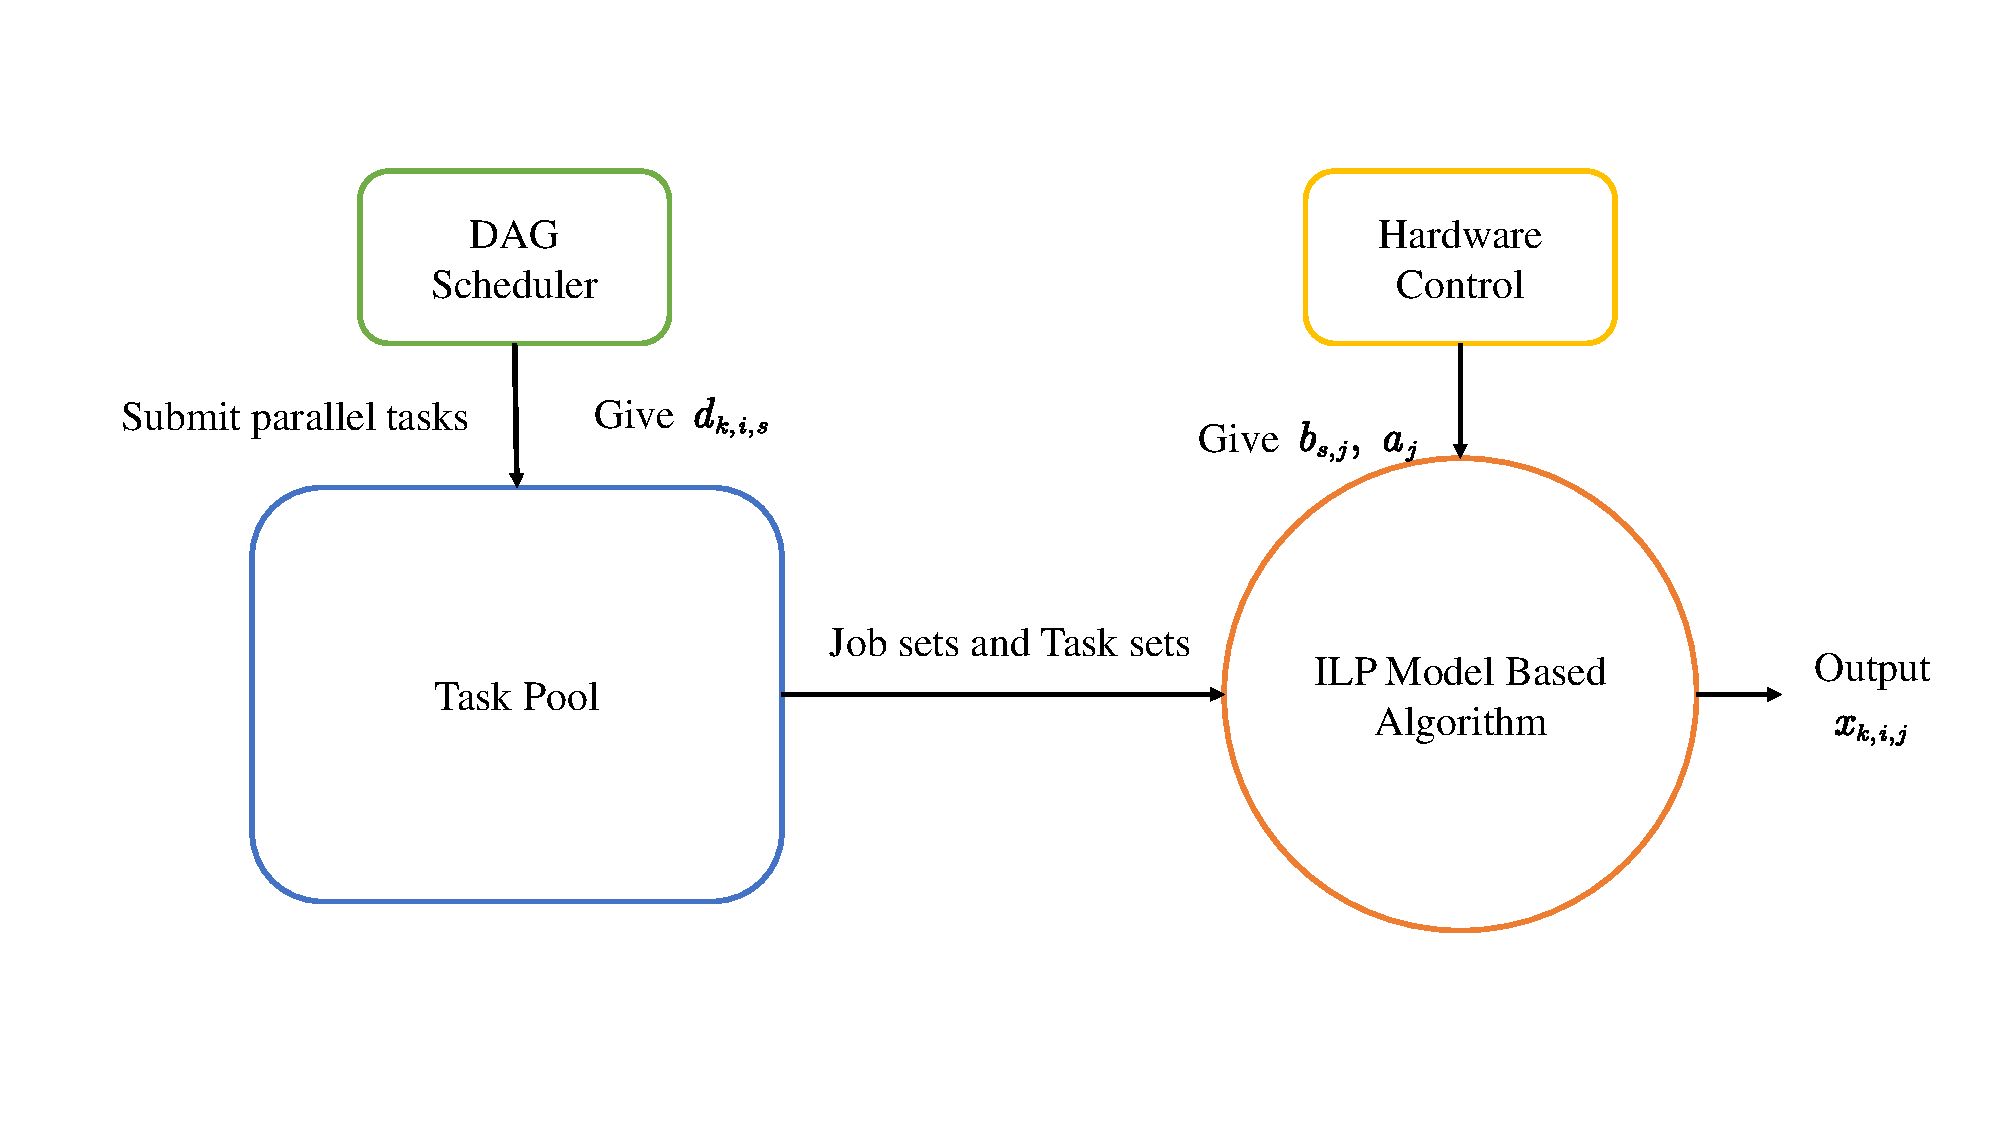
\includegraphics[width=0.8\textwidth]{Flow-Chart.pdf}
    \centering
    \caption{The Flow Chart of Precedence Constraint Relief} 
    \end{figure}

The realization of DAG scheduler is not difficult. First, by performing BFS on the DAG of each job, we can determine the depth of all jobs. Then we can store all the predecessor nodes of each task. At the beginning of scheduling, the DAG scheduler submits all tasks with the depth of 1. After that, the scheduler will loop to check whether the predecessor nodes of the remaining tasks are all completed. If all completed, then the task will be submitted to the task pool. The tasks in the pool will be scheduled by the ILP model based algorithm. This process will not be stopped until all tasks are completed.

The  pseudo code of this process is shown below:

\begin{minipage}[t]{0.8\textwidth}
    \begin{algorithm}[H]
        \BlankLine
        \caption{DAG Schedule}
        Initialize a task set $ T^{\prime} = T_1 \cup T_2 \cup \cdots \cup T_{k_n} $;\\
        Use BFS to obtain the depth $ dep_k $ for all $ k \in T^{\prime}$ in its DAG;\\
        Submit all tasks that $ dep = 1 $ to the task pool and remove them from $ T^{\prime} $;\\
        Recode the predecessor nodes of all tasks in $ T^{\prime} $;\\
        \While{$T^{\prime} \neq \varnothing$}
        {
            \If{All the predecessor nodes of $ k \in T^{\prime}$ are completed}
            {
                Submit $ k $ to the task pool;\\
                Remove $ k $ from $ T^{\prime} $;\\
            }
        }
        
    \end{algorithm}
    \end{minipage}


    So far, we have given a complete solution to the required problem.

\section{Conclusion}

In this paper, we formalized the problem, build an ILP model and come up with an algorithm based on it. We proved the NP-completeness of this problem. In addition, we also proposed a specific solution to solve the time dependence between different tasks, that is, through DAG scheduling to control the independence of tasks in the task pool.

Because we do not have enough capacity for coding, we failed to apply our algorithms to specific data by writing programs. Therefore, we cannot perform further performance analysis of the algorithm. But we implement the key part of the algorithm, which is the ILP, through c++. 

"solver.hpp" is the program to solve the ILP problem using Monte Carlo method. 







\section*{Acknowledgements}
\begin{itemize}
    \item We would like to thank Prof. Gao and Prof. Wang for their guidance to us in and after class.

    \item We give sincerely thank to TAs for their meticulous work and their valuable help to us.
    
    \item Also thank to Shanghai Jiao tong University for giving us the opportunity to communicate and cooperate together.
\end{itemize}


%
% ---- Bibliography ----
%
% BibTeX users should specify bibliography style 'splncs04'.
% References will then be sorted and formatted in the correct style.
%
% \bibliographystyle{splncs04}
% \bibliography{mybibliography}
%
\begin{thebibliography}{8}

\bibitem{ref_article2}
Y. Kwok and I. Ahmad, “Static Scheduling Algorithms for Allocating Directed Task Graphs to Multiprocessors”

\bibitem{ref_article3}
J.D.Ullman, “NP-Complete Scheduling Problem”, JOURNAL OF COMPUTER AND SYSTEM SCIENCES 10, 384--393 (1975)

\bibitem{ref_article4}
T. A. Roemer.  “A note on the complexity of the concurrent open shop problem”

\bibitem{ref_article1}
Li Chen, Shuhao Liu, Baochun Li, and Bo Li, Scheduling Jobs across Geo-Distributed Datacenters with Max-
Min Fairness, IEEE Transactions on Network Science and Engineering (TNSE), 6(3):488-500, 2019.

\end{thebibliography}
\end{document}
